%% This template can be used to write a paper for
%% Computer Physics Communications using LaTeX.
%% For authors who want to write a computer program description,
%% an example Program Summary is included that only has to be
%% completed and which will give the correct layout in the
%% preprint and the journal.
%% The `elsarticle' style is used and more information on this style
%% can be found at 
%% http://www.elsevier.com/wps/find/authorsview.authors/elsarticle.
%%
%%
\documentclass[preprint,12pt]{elsarticle}

%% Use the option review to obtain double line spacing
%% \documentclass[preprint,review,12pt]{elsarticle}

%% Use the options 1p,twocolumn; 3p; 3p,twocolumn; 5p; or 5p,twocolumn
%% for a journal layout:
%% \documentclass[final,1p,times]{elsarticle}
%% \documentclass[final,1p,times,twocolumn]{elsarticle}
%% \documentclass[final,3p,times]{elsarticle}
%% \documentclass[final,3p,times,twocolumn]{elsarticle}
%% \documentclass[final,5p,times]{elsarticle}
%% \documentclass[final,5p,times,twocolumn]{elsarticle}

%% if you use PostScript figures in your article
%% use the graphics package for simple commands
%% \usepackage{graphics}
%% or use the graphicx package for more complicated commands
%% \usepackage{graphicx}
%% or use the epsfig package if you prefer to use the old commands
%% \usepackage{epsfig}

%% The amssymb package provides various useful mathematical symbols
\usepackage{amssymb}
\usepackage{multirow}
\usepackage{amsmath}
\usepackage{bm}
\usepackage{longtable}
\usepackage{graphicx}
\usepackage{epstopdf}
\usepackage{ulem}
\usepackage[verbose]{placeins}
\usepackage{float}
\usepackage{tabularx}
\usepackage[tracking=true,spacing=true,kerning=true,final]{microtype}
\usepackage{fancyhdr}
\usepackage{geometry}
\usepackage{array}
\usepackage{lineno}
\usepackage{booktabs}
\usepackage{ragged2e}
\usepackage[utf8]{inputenc}
\usepackage[english]{babel}
\geometry{bindingoffset=0mm, left=20mm, right=20mm, top=30mm, bottom=35mm}

\newcommand{\qq}[1]{{\lq}#1{\rq}}

%% The amsthm package provides extended theorem environments
%% \usepackage{amsthm}

%% The lineno packages adds line numbers. Start line numbering with
%% \begin{linenumbers}, end it with \end{linenumbers}. Or switch it on
%% for the whole article with \linenumbers after \end{frontmatter}.
%% \usepackage{lineno}

%% natbib.sty is loaded by default. However, natbib options can be
%% provided with \biboptions{...} command. Following options are
%% valid:

%%   round  -  round parentheses are used (default)
%%   square -  square brackets are used   [option]
%%   curly  -  curly braces are used      {option}
%%   angle  -  angle brackets are used    <option>
%%   semicolon  -  multiple citations separated by semi-colon
%%   colon  - same as semicolon, an earlier confusion
%%   comma  -  separated by comma
%%   numbers-  selects numerical citations
%%   super  -  numerical citations as superscripts
%%   sort   -  sorts multiple citations according to order in ref. list
%%   sort&compress   -  like sort, but also compresses numerical citations
%%   compress - compresses without sorting
%%
%% \biboptions{comma,round}

% \biboptions{}

%% This list environment is used for the references in the
%% Program Summary
%%
\newcounter{bla}
\newenvironment{refnummer}{%
\list{[\arabic{bla}]}%
{\usecounter{bla}%
 \setlength{\itemindent}{0pt}%
 \setlength{\topsep}{0pt}%
 \setlength{\itemsep}{0pt}%
 \setlength{\labelsep}{2pt}%
 \setlength{\listparindent}{0pt}%
 \settowidth{\labelwidth}{[9]}%
 \setlength{\leftmargin}{\labelwidth}%
 \addtolength{\leftmargin}{\labelsep}%
 \setlength{\rightmargin}{0pt}}}
 {\endlist}

\journal{Computer Physics Communications}

\begin{document}

\begin{frontmatter}

%% Title, authors and addresses

%% use the tnoteref command within \title for footnotes;
%% use the tnotetext command for the associated footnote;
%% use the fnref command within \author or \address for footnotes;
%% use the fntext command for the associated footnote;
%% use the corref command within \author for corresponding author footnotes;
%% use the cortext command for the associated footnote;
%% use the ead command for the email address,
%% and the form \ead[url] for the home page:
%%
%% \title{Title\tnoteref{label1}}
%% \tnotetext[label1]{}
%% \author{Name\corref{cor1}\fnref{label2}}
%% \ead{email address}
%% \ead[url]{home page}
%% \fntext[label2]{}
%% \cortext[cor1]{}
%% \address{Address\fnref{label3}}
%% \fntext[label3]{}

\title{$ms2$: A molecular simulation tool for thermodynamic properties, release 3.0}

%% use optional labels to link authors explicitly to addresses:
%% \author[label1,label2]{<author name>}
%% \address[label1]{<address>}
%% \address[label2]{<address>}

\author[upb]{G\'{a}bor Rutkai}
\author[upb]{Andreas K\"{o}ster}
\author[upb]{Gabriela Guevara-Carrion}
\author[ltd]{Michael Schappals}
\author[hlrs]{Colin W. Glass}
\author[hlrs]{Martin Bernreuther}
\author[hlrs]{Amer Wafai}
\author[ltd]{Simon Stephan}
\author[ltd]{Maximilian Kohns}
\author[ltd]{Stephan Deublein} 
\author[ltd]{Martin Horsch}
\author[ltd]{Hans Hasse}
\author[upb]{Jadran Vrabec \corref{cor1} }

\address[upb]{Lehrstuhl f\"{u}r Thermodynamik und Energietechnik, Universit\"{a}t Paderborn, 33098~Paderborn, Germany}
\address[ltd]{Lehrstuhl f\"{u}r Thermodynamik, Universit\"{a}t Kaiserslautern, 67653 Kaiserslautern, Germany}
\address[hlrs]{H\"{o}chstleistungsrechenzentrum Universit\"{a}t Stuttgart (HLRS), 70550 Stuttgart, Germany}

\cortext[cor1]{Corresponding author: Jadran Vrabec, Warburger Str. 100, 33098 Paderborn, Germany, Tel.: +49-5251/60-2420, Email: jadran.vrabec@upb.de}

\begin{abstract}
A new version release (3.0) of the molecular simulation tool {\it ms}2 [Deublein et al., Comput. Phys. Commun. 182 (2011) 2350 and Glass et al., Comput. Phys. Commun. 185 (2014) 3302] is presented. Version 3.0 of {\it ms}2 features the implementation of two additional ensembles, i.e. microcanonical ($NVE$) and isoenthalpic–isobaric ($NpH$); the calculation of Helmholtz energy derivatives in the $NVE$ ensemble, the osmotic pressure and the Maxwell-Stefan diffusion coefficients of quaternary mixtures; thermodynamic integration as a method for calculating the chemical potential; statistics for sampling hydrogen bonds as well as the ability to execute an arbitrary number of state points in a single molecular dynamics run.

\end{abstract}

\begin{keyword}
%% keywords here, in the form: keyword \sep keyword
molecular simulation \sep molecular dynamics \sep Monte Carlo
\end{keyword}

\end{frontmatter}

%%
%% Start line numbering here if you want
%%
% \linenumbers

% Computer program descriptions should contain the following
% PROGRAM SUMMARY.

\section*{New version program summary}

\begin{small}
\noindent
{\em Program Title:} $ms2$\\

\noindent
{\em Operating system:} Unix/Linux\\

\noindent
{\em Licensing provisions(please choose one):} CC0 1.0/CC By 4.0/MIT/Apache-2.0/BSD 3-clause/BSD 2-clause/GPLv3/CC BY NC 3.0 \\

\noindent
{\em Programming language:} Fortran90\\

\noindent
{\em Has the code been vectorized or parallelized:} yes (Message Passing Interface (MPI) protocol and OpenMP
Scalability is up to 2000 cores)\\

\noindent
{\em Distribution format:} tar.gz\\

\noindent
{\em Classification:} 7.7, 7.9, 12\\

\noindent
{\em Catalogue identifiers of previous versions:} AEJF\_v1\_0 and AEJF\_v2\_0\\

\noindent
{\em Supplementary material:}\\

\noindent
{\em Journal reference of previous versions:}  S. Deublein et al., Comput. Phys. Commun. 182 (2011) 2350 and C. Glass et al., Comput. Phys. Commun. 185 (2014) 3302\\

\noindent
{\em Does the new version supersede the previous version?:} yes\\

\noindent
{\em Reasons for the new version:} introduction of new features\\

\noindent
{\em Summary of revisions:} two new ensembles ($NVE$ and $NpH$), new properties (Helmholtz energy derivatives, chemical potential via thermodynamic integration, osmotic pressure, Maxwell-Stefan diffusion coefficients of quaternary mixtures), new functionalities (detection of hydrogen bonding, the ability to execute an arbitrary number of state points in a single molecular dynamics run)\\

\noindent
{\em Nature of problem:} Calculation of application oriented thermodynamic properties: vapor-liquid equilibria of pure fluids and multi-component mixtures, thermal and caloric data as well as transport properties\\

\noindent
{\em Solution method:} Molecular dynamics, Monte Carlo, various ensembles, grand equilibrium method, Green-Kubo formalism, Lustig formalism\\

\noindent
{\em Typical running time:} varies (typically from a couple of hours up to days) depending on the specific scenario (system size, calculated properties, number of CPU cores used)\\

\noindent
{\em Restrictions:} typical problems addressed by $ms2$ are solved by simulating systems containing typically 1000 -- 5000 molecules that are modelled as rigid bodies\\

\noindent
{\em Documentation:} documentation is provided with the installation package and is available at \ead[url]{http://www.ms-2.de}\\
\end{small}


%% main text
\section{Microcanonical ($NVE$) and isoenthalpic–isobaric ($NpH$) ensembles and Helmholtz energy derivatives}
\label{sec:ensembles}

An ensemble is the set of all theoretically possible microscopic configurations (configurations on the molecular level) under specific macroscopic conditions. The microcanonical ensemble ($NVE$) is the set of all configurations that fulfill the condition of having the same number of particles $N$, volume $V$ and energy $E$, whereas the isobaric-isoenthalpic ensemble ($NpH$) represents a system at constant number of particles $N$, pressure $p$ and enthalpy $H$. Molecular dynamics (MD) mimics the time evolution of the system by numerically solving the Newton's equations of motion for all considered molecules. Because of to the nature of this solution, the time is discredized and the method yields microscopic configurations at discrete but consecutive time steps. The Monte Carlo (MC) method is the application of statistical mechanics to describe molecular systems. With this approach, microscopic configurations are generated by random numbers and potentially accepted such that only relevant and physically meaningful configurations are sampled. The generation and acceptance of these configurations is governed by specific probabilities \cite{fre02} that are ensemble-dependent and known for essentially every relevant ensemble. For MC simulations, the $NVE$ and $NpH$ ensembles were implemented in $ms2$ 3.0 according to Refs. \cite{lus98, kri05}. For MD simulations, the pressure is kept constant using Andersen's barostat \cite{and80} for the $NpH$ ensemble. Because the solution of Newton's equations of motion is approximate, the total energy of the system $E=K+U$, which consists of a kinetic $K$ (exclusively molecular velocity dependent) and potential $U$ (exclusively molecular position dependent) contribution, is not rigorously conserved in a standard MD run. Therefore, the velocity (translational and rotational) of every molecule is rescaled such that their sum calculated by the equipartition theorem matches $E-U$, where $E$ is specified and $U$ is calculated from the current configuration. For an $NpH$ run, the solution is analogous: velocities are rescaled such that the current kinetic energy $K$ matches $H-U-pV$, where $H$ and $p$ are specified, $U$ and $V$ are dependent on the current microscopic configuration. This extends the available ensembles to five:  $NVT$, $NVE$, $NpT$, $NpH$ and $\mu VT$, where $\mu$ is the chemical potential.\\ Table~\ref{tab:ensembles} contains numerical results for state points located in the dense fluid region of methyl fluoride for verification purposes.

\section{Helmholtz energy derivatives for the microcanonical ($NVE$) ensemble}
\label{sec:lustig}

Additional to the new ensembles, the calculation of the Helmholtz energy derivatives 
\begin{equation} 
A^\text{r}_{nm}=(1/T)^n \rho^m \frac{\partial^{n+m}f^\text{r}(T,\rho)/(RT)}{\partial(1/T)^n \partial \rho^m},
\label{eq:helmholtzderiv}
\end{equation}
with the molar residual Helmholtz energy $f^\text{r}$, the temperature $T$, the density $\rho$, the molar gas constant $R$ were also introduced for the $NVE$ ensemble up to the order $n=3$ and $m=2$. It can be shown that the total reduced Helmholtz energy $f/(RT)$ can be additively separated into an ideal $f^\text{o}/(RT)$ and a residual contribution $f^\text{r}/(RT)$. The ideal contribution by definition corresponds to the value of $f/(RT)$ when no intermolecular interactions are at work \cite{spa00}. $f^\text{o}/(RT)$ consist of an exclusively temperature and an exclusively density dependent part. The former has a trivial density dependence $\ln(\rho/\rho_\text{ref})$, whereas the latter has a non-trivial temperature dependence. The formalism that allows for the calculation of these derivatives on the fly from a single simulation run per state point was published by Lustig \cite{lus11, lus12} and was already introduced for the $NVT$ ensemble in the previous release. $ms2$ 3.0 now yields these derivatives also for $NVE$ simulations. Here, however, in contrast to $NVT$ simulations, there are two numerical results for each calculated derivative $A_{nm}$ which is due to the two possible entropy definitions in statistical mechanics \cite{lus12}. In any case, these two different sets of results must be identical in the thermodynamic limit ($N \longrightarrow \infty$). In practice, they already agree within their estimated statistical uncertainty for a simulation with around a thousand particles.\\
A detailed description of how to convert these derivatives to common thermodynamic properties are provided in the supplementary material of release 2.0 of Ref. \cite{ms2_2.0} and in Ref. \cite{spa00}.

\begin{table}
  \centering
  \caption{Comparison of the ensembles implemented in \textit{ms}2 for a dense liquid state point of Methyl Fluoride (R41). Statistical uncertainties were estimated with the method of Flyvbjerg and Petersen \cite{fly89}}
    \begin{tabular}{rrllll}
    \hline
          &       & Temperature & Density & Pressure & Potential energy \\
          &       & K   & mol/l & MPa & kJ/mol \\
    \hline
    \multicolumn{1}{c}{\multirow{4}[0]{*}{MD}} & \multicolumn{1}{l}{\textit{NVT}} & 220   & 27    & 100.2 $\pm$ 0.2 & -16.63 $\pm$ 0.02 \\
    \multicolumn{1}{c}{} & \multicolumn{1}{l}{\textit{NpT}} & 220   & 26.994 $\pm$ 0.005 & 100   & -16.65 $\pm$ 0.04 \\
    \multicolumn{1}{c}{} & \multicolumn{1}{l}{\textit{NVE}} & 220.09 $\pm$ 0.06 & 27    & 100.1 $\pm$ 0.2 & -16.63 $\pm$ 0.01 \\
    \multicolumn{1}{c}{} & \multicolumn{1}{l}{\textit{NpH}} & 219.8   $\pm$ 0.2 & 26.991 $\pm$ 0.004 & 100   & -16.64 $\pm$ 0.03 \\
          & \multicolumn{1}{l}{\textit{}} &       &       &       &  \\
    \multicolumn{1}{c}{\multirow{4}[0]{*}{MC}} & \multicolumn{1}{l}{\textit{NVT}} & 220   & 27    & 100.2 $\pm$ 0.1 & -16.66 $\pm$ 0.01 \\
    \multicolumn{1}{c}{} & \multicolumn{1}{l}{\textit{NpT}} & 220   & 27.015 $\pm$ 0.002 & 100   & -16.66 $\pm$ 0.02 \\
    \multicolumn{1}{c}{} & \multicolumn{1}{l}{\textit{NVE}} & 220.01 $\pm$ 0.03 & 27    & 100.2 $\pm$ 0.1 & -16.65 $\pm$ 0.01 \\
    \multicolumn{1}{c}{} & \multicolumn{1}{l}{\textit{NpH}} & 220.11 $\pm$ 0.04 & 27.005 $\pm$ 0.002 & 100   & -16.66 $\pm$ 0.01 \\
    \hline
    \end{tabular}%
  \label{tab:ensembles}%
\end{table}%

\section{Thermodynamic integration}
\label{sec:thermoint}

The previously described method of Lustig does not allow for the direct sampling of the chemical potential thus entropic properties like $A_{00}$. Such an effort still requires techniques based on free energy calculation such as particle insertion and/or thermodynamic integration \cite{fre02}. Widom's particle insertion method \cite{wid63} is a conceptually straightforward approach to calculate the chemical potential with low computational cost, both for pure substances and mixtures. The total chemical potential for a particle $i$ can be separated into an ideal (o) and a residual (r) contribution the same way as the Helmholtz energy is decomposed (cf. section~\ref{sec:ensembles}). $\mu^\text{total}_{i} (T,\rho,x_i) = \mu^\text{o}_{i}(T) + RT \ln (N_i/V/\rho_\text{ref}) + \mu^{r}_{i} (T,\rho,x_i)$, where $N_i$ is the number of particles with the same chemical identity that of $i$, $\rho=N/V$, $x_i=N_i/N$ and $\rho_\text{ref}$ is an arbitrary reference density. The part $\mu^\text{total}_{i} - \mu^{o}_{i}(T)$ is often referred to as the configurational chemical potential $\mu^\text{conf}_{i}$. Widom's method requires the frequent insertion of an additional $(i=N+1)$ molecule into the simulation volume at a random position with a random orientation. At constant temperature and constant pressure or volume the potential energy $U_i$ of this test molecule, the interaction energy with all other "real" $N$ molecules, yields the configurational chemical potential according to
\begin{equation}
\mu^\text{conf}_{i}=\mu^\text{total}_{i}-\mu^{\text{o}}_{i}\left(T\right)=-k_{\text{B}}T \ln \frac{\left\langle V \exp \left(-U_i/k_{\text{B}}T\right)\right\rangle}{\left\langle N_{i}\right\rangle},
\label{eq:widom}
\end{equation}
where $k_\text{B}$ is Boltzmann's constant. The test molecule is removed immediately after the calculation of its potential energy $U_i$, thus it does not influence the properties of the system in any way. In contrast to the usual convention, the brackets $<>$ here have a dual meaning: They stand for either $NVT$ or $NpT$ ensemble average as well as an integral over all possible positions and orientations of the test molecule added to the system. The density of the system has a significant influence on the accuracy of this method. For state points with a high density, test molecules almost always overlap with real molecules, which leads to a potential energy $U_i \rightarrow \infty$ and thus to a vanishing contribution to Eq.~(\ref{eq:widom}), resulting in poor statistics and often even to complete failure of sampling.\\
Thermodynamic integration is one solution to overcome the limitations of Widom's particle insertion method. The idea behind calculating the chemical potential by thermodynamic integration is to avoid insertion of the test particle in system $A$ and perform it in system $B$ for which it is not problematic. Since the chemical potential is a state variable, its change $\mu_A-\mu_B$ can be calculated using any arbitrary path between states $A$ and $B$. This path is represented by the parameter $\lambda$. It can be shown \cite{fre02} that the relation between $\lambda$ and $\mu_A-\mu_B$ is 
\begin{equation}
\mu_{A,i}-\mu_{B,i}=\int_{B(\lambda_\text{min})}^{A(\lambda_\text{max})} \left\langle \frac{\partial U_i(\lambda)}{\partial \lambda} \right\rangle d \lambda 
\label{eq:thermoint}
\end{equation}
for particle $i$. The bracket $<>$ in this equation denotes $NVT$ or $NpT$ ensemble average and $U_i$ is the potential energy of particle $i$ that must be a part of the system the same way as the other particles are. The only difference between $i$ and normal particles is that the interaction energy $U_i(\lambda)$ is scaled between states $A(\lambda_\text{max})$ and $B(\lambda_\text{min})$ with $\lambda$. As long as $\partial U_i(\lambda)/\partial \lambda$ can be calculated analytically and sampled during simulation, the actual way of scaling $U_i(\lambda)$ with $\lambda$ can be chosen arbitrarily because $\mu$ is a state variable. The integration with respect to $\lambda$ is evaluated numerically. Assuming that $\mu_{B,i}$ is practically zero or at least can be successfully calculated by Widom’s particle insertion method at the end point $B$ using Eq.~\eqref{eq:widom}, $\mu_{B,i}$ yields the configurational part of the total chemical potential. The non-linear scaling $U_i(\lambda)=\lambda^x U_i$ for $\lambda_\text{min} \leq \lambda \leq 1$ with an adaptive sampling technique \cite{kri07} was implemented for MC with $x$ and $\lambda_\text{min}$ being input parameters. This adaptive technique allows for the sampling of the entire range of $\lambda_\text{min} \leq \lambda \leq 1$ in a single MC simulation run with arbitrary resolution for the numerical integration. Besides the standard $NVT$ and $NpT$ ensemble MC moves, the simulation includes changes of $\lambda$ controlled by a proper MC acceptance criterion ensuring visits at each discrete $\lambda$ value in the range $\lambda_\text{min} \leq \lambda \leq 1$. For MD simulations, changes of $\lambda$ are carried out also on the fly in a single simulation but without any acceptance criterion. A detailed description of the parameter setup for is in the supplementary material. \\

\section{Quaternary Maxwell-Stefan diffusion coefficients}
\label{sec:quat}

$ms2$ employs the Green-Kubo formalism based on the net velocity auto-correlation function to obtain $n\times n$ phenomenological coefficients~\cite{kri05b}  

\begin{equation}\label{MS_lamda}
L_{ij}= \frac{1}{3N}\int_0 ^{\infty} \rm{d}t~\Big\langle\sum_{{\it k}=1}^{{\it N_i}} \mathbf{v}_{\it i,k}(0)\cdot\sum_{{\it l}=1}^{{\it N_{j}}} \mathbf{v}_{\it j,l}(t)\Big\rangle \,,% \di,
\end{equation}

\noindent in a mixture of $n$ components. Here, $N$ is the total number of molecules, $N_{i}$ is the number of molecules of component $i$ and $\mathbf{v}_{i,k}(t)$ denotes the center of mass velocity vector of the $k$-th molecule of component $i$ at time $t$. Note that Eq.~\eqref{MS_lamda} corresponds to a reference frame in which the mass-averaged mixture velocity is zero~\cite{kri05b}.

Starting from the phenomenological coefficients $L_{ij}$, the elements of a $(n-1) \times (n-1)$ matrix $\bm{\Delta}$ can be defined as~\cite{kri05b}

\begin{equation}
 \Delta_{ij} = (1-x_i)\left(\frac{L_{ij}}{x_j}-\frac{L_{in}}{x_n}\right)-x_i\sum^{n}_{k=1\neq i}\left(\frac{L_{kj}}{x_j}-\frac{L_{kn}}{x_n}\right),
\end{equation} 

\noindent so that its inverse matrix $\bm{B} = \bm{\Delta}^{-1}$ is related to the Maxwell-Stefan diffusion coefficients $\textit{\DJ}_{ij}$. In the case of a quaternary mixture, the six Maxwell-Stefan diffusion coefficients are then given by~\cite{kri05b}

\begin{align}
{\textit{\DJ}_{14}}&=\frac{1}{B_{11}+(x_2/x_1)B_{12}+(x_3/x_1)B_{13}},\\
{\textit{\DJ}_{24}}&=\frac{1}{B_{22}+(x_1/x_2)B_{21}+(x_3/x_2)B_{23}},\\
{\textit{\DJ}_{34}}&=\frac{1}{B_{33}+(x_1/x_3)B_{31}+(x_2/x_3)B_{32}},\\
{\textit{\DJ}_{12}}&= \frac{1}{1/{\textit{\DJ}_{24}}-B_{21}/{x_2}},\\
{\textit{\DJ}_{13}}&= \frac{1}{1/{\textit{\DJ}_{14}}-B_{13}/{x_1}},\\
{\textit{\DJ}_{14}}&= \frac{1}{1/{\textit{\DJ}_{24}}-B_{23}/{x_2}},\\
\end{align}

\noindent where $x_i$ is the mole fraction of component $i$.

\section{Hydrogen bonding}
\label{sec:Hydrogen bonding}

There is no unambiguous characterization of a hydrogen bond between two molecules \cite{Stillinger80, HI10, ADKSSACCDHKLMN11}. Rather, the hydrogen (H)~bond \qq{is a structural motif and involves at least three atoms} \cite{TK06}. The International Union of Pure and Applied Chemistry (IUPAC) defines the hydrogen bond as \qq{an attractive interaction between a hydrogen atom from a molecule or molecular fragment X--H in which X is more electronegative than H, and an atom or a group of atoms in the same or a different molecule, in which there is evidence of bond formation} \cite{ADKSSACCDHKLMN11}.

Energetic \cite{Stillinger80}, geometric \cite{Haughney1987}, and topological \cite{HI10} hydrogen bonding criteria have been proposed in the literature. Geometric criteria, which are not overly complex, are often based on the following assumptions \cite{RMHH12}:
\begin{itemize}
	\item The interaction between two hydrogen bonded sites is highly directional and short ranged.
	\item A donor interacts at most with a single acceptor, an acceptor can interact with multiple donors.
\end{itemize}
Accordingly, a class of geometric criteria for the evaluation of hydrogen bonding networks in fluids was implemented in \textit{ms}2. Thereby, the triangle between three charge sites, being part of two molecules, is evaluated to determine whether an interaction between two sites constitutes a hydrogen bond or not. A molecule acts as a donor to another molecule, the acceptor, if the following conditions hold \cite{Haughney1987, RMHH12, LC93, CC06}:
\begin{itemize}
	\item{} The distance between the donor and the acceptor is smaller than the respective threshold distance, i.e.\ $\ell_\mathrm{AD}$ or $\ell_\mathrm{DA}$, cf.\ Fig.\ \ref{fig:Hbonding}.
        \item{} The distance between the acceptor sizes of the acceptor and donor molecules is smaller than $\ell_\mathrm{AA}$.
        \item{} The angle between the acceptor-donor axis and the acceptor-acceptor axis is smaller than the respective threshold angle, i.e.\ $\varphi_\mathrm{DAA}$ or $\varphi_\mathrm{AAD}$, cf.\ Fig.\ \ref{fig:Hbonding}. 
\end{itemize}
Therein, $\ell_\mathrm{AD}$, $\ell_\mathrm{DA}$, $\ell_\mathrm{AA}$, $\varphi_\mathrm{DAA}$, and $\varphi_\mathrm{AAD}$ are the parameters of the implemented class of hydrogen bonding criteria; for methanol, e.g., Haughney \textit{et al.}\ \cite{Haughney1987} use $\ell_\mathrm{AD} = \ell_\mathrm{DA} = 2.6$ \AA{}, $\ell_\mathrm{AA} = 3.5$ \AA, and $\varphi_\mathrm{AAD}= \varphi_\mathrm{DAA} = 30^\circ$.
Beside methanol \cite{Haughney1987}, such geometric criteria have been applied to a variety of fluids, in particular to water \cite{LC93, CC06, LC96}, methanol-water mixtures \cite{CC14}, and ethanol \cite{RMHH12, SPG97, XYH09}, including previous molecular simulations with an unreleased development version of the \textit{ms}2 program \cite{RMHH12}. Hydrogen bonds in sorbate-sorbent interactions can be treated analogously \cite{BKS14}. For hydrogen fluoride, a simple distance-based criterion can be used \cite{KBMP03}, which is also covered by the present implementation. A detailed description of the parameter setup is in the supplementary material. 

\begin{figure}[htb]
	\centering
	\def\svgwidth{\textwidth}
	%\input{Abb_HBonding.tex} 
	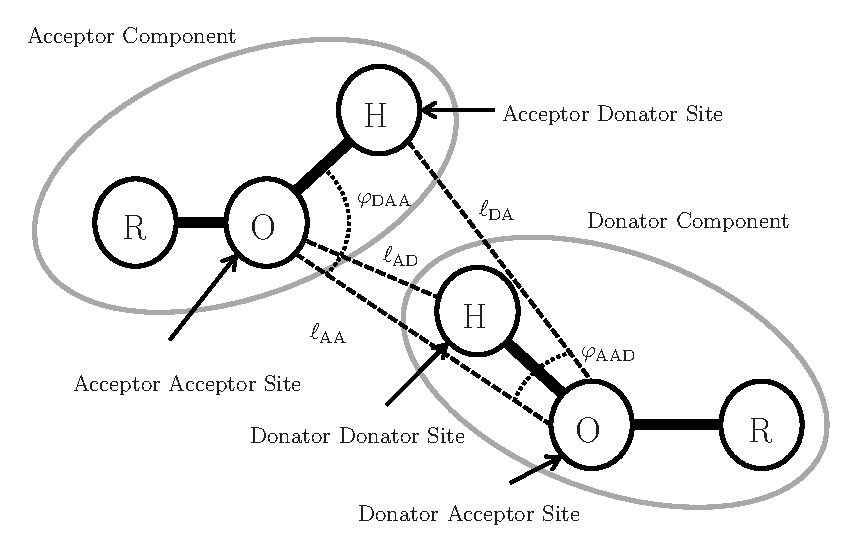
\includegraphics[width=0.5\textwidth]{HBonding.eps}
	\caption{Hydrogen bonding criteria implemented in the present release version of \textit{ms}2.}
	\label{fig:Hbonding}
\end{figure}




%% The Appendices part is started with the command \appendix;
%% appendix sections are then done as normal sections
%% \appendix

%% \section{}
%% \label{}

%% References
%%
%% Following citation commands can be used in the body text:
%% Usage of \cite is as follows:
%%   \cite{key}         ==>>  [#]
%%   \cite[chap. 2]{key} ==>> [#, chap. 2]
%%

%% References with bibTeX database:

\bibliography{biblio}
\bibliographystyle{elsarticle-num}
%% Authors are advised to submit their bibtex database files. They are
%% requested to list a bibtex style file in the manuscript if they do
%% not want to use elsarticle-num.bst.

%% References without bibTeX database:

% \begin{thebibliography}{00}

%% \bibitem must have the following form:
%%   \bibitem{key}...
%%

% \bibitem{}

% \end{thebibliography}


\end{document}

%%
%% End of file 